% !TeX spellcheck = en_US
% !TeX encoding = UTF-8
\documentclass[11.5pt,aspectratio=1610,xcolor={usenames,dvipsnames,table}]{beamer}
\mode<presentation>
\usepackage[T1]{fontenc}
\usepackage[utf8]{inputenc}
\usepackage[english]{babel}
\usepackage{lmodern}
\usepackage[babel,style=english,english=american]{csquotes}
\usepackage{mathabx}
\usepackage{latexsym}
\usepackage{graphicx}
\usepackage{multicol}
\usepackage{multirow}
\usepackage[gen]{eurosym}
\usepackage{pgfpages}
\usepackage{xspace}
\usepackage{appendixnumberbeamer}
\usepackage[binary-units]{siunitx}
\usepackage{tabu}
\usepackage{graphicx}
\usepackage{pgfgantt}
%\usepackage{biblatex}

%\setcounter{tocdepth}{2}

%\usetheme[numbering=counter,progressbar=frametitle]{metropolis}
%\usetheme[numbering=none]{metropolis}
\usetheme[sectionpage=none,subsectionpage=none,numbering=counter,progressbar=none]{metropolis}
\usepackage{bibentry}
\usepackage[justification=centering]{caption}
%\usepackage[square,numbers]{natbib}
\definecolor{brsu_blue}{HTML}{0BA1E2}
\usepackage{url}
\setbeamercolor{title separator}{fg=brsu_blue}
\setbeamercolor{progress bar}{fg=brsu_blue}
\setbeamercolor{normal text}{fg=black,bg=white}
\setbeamercolor{frametitle}{bg=brsu_blue,fg=white}

\title{Read Digits from Natural Images using Convolutional Neural Network}

%\titlegraphic{\includegraphics[width=5cm]{gfx/logo}}

\author{Ramesh Kumar \\ Roberto Cai Wu}

\date{\today}

\setbeamertemplate{caption}{\raggedright\insertcaption\par}



\setbeamerfont{footnote}{size=\tiny}






\begin{document}

\begin{frame}
\titlepage
\end{frame}


\section{Motivation}
\begin{frame}
	\frametitle{ Motivation}
	\begin{itemize}
		\item This is a optical character recognition (OCR) problem
		\item Digit recognition is used in various applications such as postal mail
		sorting, bank check processing, form data entry, etc
		\item Digit recognition is an important component of modern-day map making \cite{Goodfellow2013}
		%\item It is a challenging problem due to:  \cite{Goodfellow2013}
		
	\end{itemize}
\end{frame}

\section{Problem Description}
\begin{frame}
\frametitle{Problem Description}
\begin{itemize}
	\item To read digits from natural images 
	\item We use convolutional neural networks(CNN) for fast processing, accuracy and speed
\end{itemize}

\end{frame}


\section{Challenges}
\begin{frame}
\frametitle{Challenges}
\begin{itemize}
	\item Wide variability of visual appearance of text: fonts, colors, and orientations \cite{Goodfellow2013}
	\item Different environmental factors: lightning, shadows, and occlusions \cite{Goodfellow2013}
	\item Image acquisition factors: motion, blurring, and resolution \cite{Goodfellow2013}
	%\item May be more too
\end{itemize}
\end{frame}

%% 2nd paper %%

%\begin{frame}

%\frametitle{Assumptions and Pre-requistes
%}
%\begin{itemize}
%	\item 
%\end{itemize}
%\end{frame}

\section{Methodology}
\begin{frame}

\frametitle{Methodology}
%\myheading{\textbf{Block Diagram}}

\begin{itemize}
	\item Load and Interpret DataSet(done)
	\item Pre-processing(started)
	\item Convolutional Neural Network(started reading)
	\item Post-processing(yet to start)
\end{itemize}
\begin{figure}[!h]
	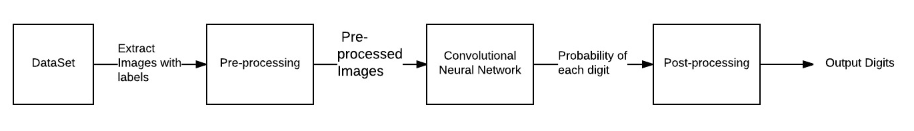
\includegraphics[width=\textwidth ]{block_diagram.png}
	\caption{Block Diagram of System}
\end{figure}

\end{frame}

%% 

\begin{frame}

\frametitle{DataSet}

\begin{figure}[!h]
	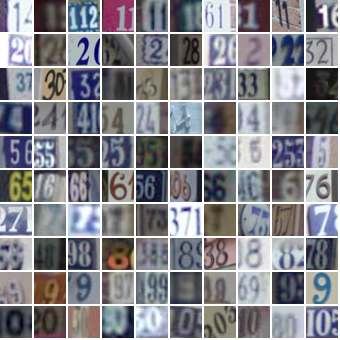
\includegraphics[width=\textwidth, height = 5cm]{dataset.png}
	\caption{Street View House Numbers Data set \cite{SVHN}}
\end{figure}

\end{frame}

\begin{frame}

\frametitle{Pre-processing}

\begin{figure}[!h]
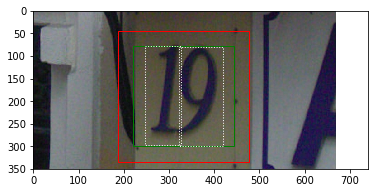
\includegraphics[width=\textwidth]{19.png}
\caption{Example }

\end{figure}
\end{frame}

\begin{frame}

\frametitle{Convolutional Neural Network(CNN)}

\begin{itemize}
	\item State-of-the-art shows CNN performs better as compare to other approaches\cite{cnn}
	\item Extracts features from the images and classify them
	\item Three type of Layers
		\begin{itemize}
			\item Convolutional: Extract low-level and high-level features
			\item Pooling: Reduce amount of parameters and computations
			\item Fully Connected: Neurons are fully connected
		\end{itemize}	
	\begin{figure}[!h]
		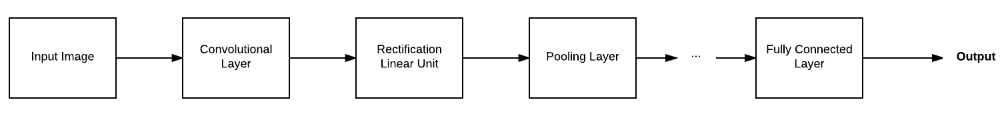
\includegraphics[width=\textwidth]{cnn.png}
		\caption{Basic Architecture of CNN }
		
	\end{figure}

\end{itemize}
\end{frame}

%% post processing

\begin{frame}
\frametitle{Post-processing}

\begin{itemize}
	\item Combine digits and show complete output
\end{itemize}

\end{frame}

\begin{frame}
\frametitle{Testing \& Evaluation}

\begin{itemize}
	\item Consider maximum digits in image are 5
	\item Test the images of digits from live camera under different conditions
	\item Use validation set from dataset to compute accuracy of model
\end{itemize}
\end{frame}

\bibliographystyle{unsrt}
\nocite*
\bibliography{presentation.bib}

%\begin{thebibliography}{9}
%\bibitem{MdArfat}
%Md Arafat Sultan, Cristobal Salazar and Tamara Sumner, "Fast and Easy Short Answer Grading with High Accuracy", Conference of the North American Chapter of the Association for Computational Linguistics: Human Language Technologies, San Diego California, USA, June 12-17, 2016
%\bibitem{Sultan_wordAligner}"Md Arafat Sultan
%	, Steven Bethard and Tamara Sumner", "Back to Basics for Monolingual Alignment: Exploiting Word Similarity and
%	Contextual Evidence",  TACL, 2014
%
%\bibitem{Nlp}
%Speech and Language Processing by Daniel Jurafsky and James H. Martin
%\bibitem{lemmaAndStemma}
% https://queryunderstanding.com/stemming-and-lemmatization-6c086742fe45
%
%\bibitem{n-gram}
% http://www.dictionary.com/browse/n-gram
%
%
%\end{thebibliography}


\end{document}
